%==================================================================================
%==================================================================================
% Document		:		Chapitre: Evaluation de résumé automatique du texte
%----------------------------------------------------------------------------------
%
% Auteur		: 		Abdelkrime ARIES
% Établissement	:		ESI (Ecole Nationale Supérieure d'Informatique; ex. INI) 
% Adresse		:		Oued Smar, Alger, Algérie 
% Année			:		2012/2013
% Thèse			:		Magister
% discipline 	:		Informatique 
% Spécialité	:		IRM (Informatique Répartie et Mobile)
% Titre			:		Résumé automatique de textes
%
%==================================================================================
%==================================================================================

%==========================L'entete de chapitre====================================
%==================================================================================
 \ifx\wholebook\relax\else
  	\documentclass[a4paper,12pt,oneside]{../use/ESIthesis}
  	
  	\usepackage{amsmath,amssymb}             % AMS Math
\usepackage[utf8]{inputenc}
%\usepackage[T1]{fontenc} %,LAE 
\usepackage[T1]{fontenc}
%\usepackage[french,english]{babel}
\usepackage[frenchb]{babel}
\usepackage{microtype}

%\usepackage[left=2.5cm,right=2.5cm,top=2.5cm,bottom=2.5cm,includefoot,includehead,headheight=13.6pt]{geometry}
\usepackage[left=2.8cm,right=2.2cm,top=2.8cm,bottom=2.8cm,includefoot,includehead,headheight=13.6pt]{geometry}
%\usepackage[left=3.8cm,right=3.2cm,top=2.8cm,bottom=2.8cm,includefoot,includehead,headheight=13.6pt]{geometry}
%\usepackage[left=1.5in,right=1.3in,top=1.1in,bottom=1.1in,includefoot,includehead,headheight=13.6pt]{geometry}
\renewcommand{\baselinestretch}{1.5}

% Table of contents for each chapter

\usepackage[nottoc, notlof, notlot]{tocbibind}
\usepackage[french]{minitoc}
\setcounter{minitocdepth}{1}
\mtcindent=15pt
% Use \minitoc where to put a table of contents

\usepackage{aecompl}

% Glossary / list of abbreviations

\usepackage[intoc]{nomencl}
%\renewcommand{\nomname}{List of Abbreviations}

\makenomenclature

% My pdf code

\usepackage[pdftex]{graphicx}
\usepackage[a4paper,pagebackref,hyperindex=true]{hyperref}

%I added
%\usepackage{tabulary}
%\usepackage{longtable}
%\usepackage[table]{xcolor}
\usepackage{indentfirst}


% Links in pdf
\usepackage{color}
%\definecolor{linkcol}{rgb}{0,0,0.4} 
%\definecolor{citecol}{rgb}{0.5,0,0} 

% Change this to change the informations included in the pdf file

% See hyperref documentation for information on those parameters

\hypersetup
{
%bookmarksopen=true,
pdftitle=Résumé Automatique de Textes,
pdfauthor=Abdelkrime ARIES, 
pdfsubject= {Résumé automatique de textes en utilisant une approche statistique, le regroupement, et la classification} , %subject of the document
%%pdftoolbar=false, % toolbar hidden
%pdfmenubar=true, %menubar shown
%pdfhighlight=/O, %effect of clicking on a link
colorlinks=false, %couleurs sur les liens hypertextes
%pdfpagemode=None, %aucun mode de page
%pdfpagelayout=SinglePage, %ouverture en simple page
%pdffitwindow=true, %pages ouvertes entierement dans toute la fenetre
%linkcolor=linkcol, %couleur des liens hypertextes internes
%citecolor=citecol, %couleur des liens pour les citations
%urlcolor=linkcol %couleur des liens pour les url
}



% Some useful commands and shortcut for maths:  partial derivative and stuff

\newcommand{\pd}[2]{\frac{\partial #1}{\partial #2}}
\def\abs{\operatorname{abs}}
\def\argmax{\operatornamewithlimits{arg\,max}}
\def\argmin{\operatornamewithlimits{arg\,min}}
\def\diag{\operatorname{Diag}}
\newcommand{\eqRef}[1]{(\ref{#1})}

\usepackage{rotating}                    % Sideways of figures & tables
%\usepackage{bibunits}
%\usepackage[sectionbib]{chapterbib}          % Cross-reference package (Natural BiB)
%\usepackage{natbib}                  % Put References at the end of each chapter
                                         % Do not put 'sectionbib' option here.
                                         % Sectionbib option in 'natbib' will do.
\usepackage{fancyhdr}                    % Fancy Header and Footer

\usepackage{txfonts}                     % Public Times New Roman text & math font
  
%%% Fancy Header %%%%%%%%%%%%%%%%%%%%%%%%%%%%%%%%%%%%%%%%%%%%%%%%%%%%%%%%%%%%%%%%%%
% Fancy Header Style Options

\pagestyle{fancy}                       % Sets fancy header and footer
\fancyfoot{}                            % Delete current footer settings

%\renewcommand{\chaptermark}[1]{         % Lower Case Chapter marker style
%  \markboth{\chaptername\ \thechapter.\ #1}}{}} %

%\renewcommand{\sectionmark}[1]{         % Lower case Section marker style
%  \markright{\thesection.\ #1}}         %
%\fancyhead[LE,RO]{\bfseries\thepage}    % Page number (boldface) in left on even
%										% pages and right on odd pages
%\fancyhead[RE]{\bfseries\nouppercase{\leftmark}}      % Chapter in the right on even pages
%\fancyhead[LO]{\bfseries\nouppercase{\rightmark}}     % Section in the left on odd pages

\fancyhead[R]{\bfseries\thepage}    % Page number (boldface) in right
\fancyhead[L]{\bfseries\nouppercase{\rightmark}}     % Section in the left on odd pages

\let\headruleORIG\headrule
\renewcommand{\headrule}{\color{black} \headruleORIG}
\renewcommand{\headrulewidth}{1.0pt}
\usepackage{colortbl}
\arrayrulecolor{black}

\fancypagestyle{plain}{
  \fancyhead{}
  \fancyfoot{}
  \renewcommand{\headrulewidth}{0pt}
}

%\usepackage{algorithm}
%\usepackage[noend]{algorithmic}

%%% Clear Header %%%%%%%%%%%%%%%%%%%%%%%%%%%%%%%%%%%%%%%%%%%%%%%%%%%%%%%%%%%%%%%%%%
% Clear Header Style on the Last Empty Odd pages
\makeatletter

\def\cleardoublepage{\clearpage\if@twoside \ifodd\c@page\else%
  \hbox{}%
  \thispagestyle{empty}%              % Empty header styles
  \newpage%
  \if@twocolumn\hbox{}\newpage\fi\fi\fi}

\makeatother
 
%%%%%%%%%%%%%%%%%%%%%%%%%%%%%%%%%%%%%%%%%%%%%%%%%%%%%%%%%%%%%%%%%%%%%%%%%%%%%%% 
% Prints your review date and 'Draft Version' (From Josullvn, CS, CMU)
\newcommand{\reviewtimetoday}[2]{\special{!userdict begin
    /bop-hook{gsave 20 710 translate 45 rotate 0.8 setgray
      /Times-Roman findfont 12 scalefont setfont 0 0   moveto (#1) show
      0 -12 moveto (#2) show grestore}def end}}
% You can turn on or off this option.
% \reviewtimetoday{\today}{Draft Version}
%%%%%%%%%%%%%%%%%%%%%%%%%%%%%%%%%%%%%%%%%%%%%%%%%%%%%%%%%%%%%%%%%%%%%%%%%%%%%%% 

\newenvironment{maxime}[1]
{
\vspace*{0cm}
\hfill
\begin{minipage}{0.5\textwidth}%
%\rule[0.5ex]{\textwidth}{0.1mm}\\%
\hrulefill $\:$ {\bf #1}\\
%\vspace*{-0.25cm}
\it 
}%
{%

\hrulefill
\vspace*{0.5cm}%
\end{minipage}
}

\let\minitocORIG\minitoc
\renewcommand{\minitoc}{\minitocORIG \vspace{1.5em}} %1.5em

\usepackage{multirow}
%\usepackage{slashbox}

\newenvironment{bulletList}%
{ \begin{list}%
	{$\bullet$}%
	{\setlength{\labelwidth}{25pt}%
	 \setlength{\leftmargin}{30pt}%
	 \setlength{\itemsep}{\parsep}}}%
{ \end{list} }

\newtheorem{definition}{Définition }
\renewcommand{\epsilon}{\varepsilon}

% centered page environment

\newenvironment{vcenterpage}
{\newpage\vspace*{\fill}\thispagestyle{empty}\renewcommand{\headrulewidth}{0pt}}
{\vspace*{\fill}}

%%%%%%%%%%%%%%%%%%%%%%%%%%%%%%%%%%%%%%%%%%%%%%%%%%%%%%%%%%%%%%%%%%%%
% Par Karim
%%%%%%%%%%%%%%%%%%%%%%%%%%%%%%%%%%%%%%%%%%%%%%%%%%%%%%%%%%%%%%%%%%%%
%for the degree sign
\usepackage{textcomp} 
\usepackage{bookmark}
\usepackage{framed}
\usepackage{arabtex}
%\usepackage{nashbf}
%\usepackage{atrans}
%calligra font for the remerciement
\usepackage{calligra}

%List of acronyms
\usepackage{acronym}

\newcommand{\racine}{./}

\newcommand{\setracine}[1]{\renewcommand{\racine}{#1}}

\newcommand{\tablefile}[1]{\input{\racine tab/#1}}
\newcommand{\appendixfile}[1]{\input{\racine anx/#1}}
%\newcommand{\chapterfile}[1]{\input{\racine chap/#1}}

\newcommand{\stitle}[1]{
\noindent
\textbf{#1}
}

\newenvironment{itemizeb}
{\begin{list}{\textbullet} {\setlength{\rightmargin}{0cm} \setlength{\leftmargin}{1cm}}}
{\end{list}}


\newenvironment{itemizec}
{\begin{list}{\textopenbullet} {\setlength{\rightmargin}{0cm} \setlength{\leftmargin}{1cm}}}
{\end{list}}


\newcommand{\kexpbox}[1]{

\vspace{5mm}
\noindent
 \fbox{%
   \parbox{0.985\linewidth}{%
   \vspace{2mm}
   {\large  \textbf{Exemple:}}\\
      #1
   }%
 }
}

\newcommand{\kbox}[1]{

\vspace{2mm}
\noindent
 \fbox{%
   \parbox{0.965\linewidth}{%
   \vspace{2mm}
      #1
   }%
 }
}

\newenvironment{kexp}
{
\begin{framed}
\noindent
{\large  \textbf{Exemple:}}\\
}
{
\end{framed}
}

%%%%%%%%%%%%%%%%%%%%%%%%%%%%%%%%%%%%%%%%%%%%%%%%%%%%%%%%%%%%%%%%%%%%
%%%%%%%%%%%%%%%%%%%%%%%%%%%%%%%%%%%%%%%%%%%%%%%%%%%%%%%%%%%%%%%%%%%%

% definitions.
% -------------------

\setcounter{secnumdepth}{3}
\setcounter{tocdepth}{2}

\newcommand{\tab}[1]{{\hskip #1}}
  	 	
  	 	\setracine{../}
  	 	\graphicspath{{.}{../fig/}}
  	 	
  	 	\begin{document}
  	 	
  	 	\dominitoc 
  	 	\selectlanguage {francais}
  	 	%just to create the .toc file, then you can hide it
  	 	%\tableofcontents
  	 	\mainmatter
  \fi
%==================================================================================

\chapter{Évaluation du résumé automatique de textes}
\label{chap:evalRAT}
\minitoc

\section{Introduction}

Pour évaluer l'efficacité d'un système de résumé automatique, il n'existe pas un protocole unifié, mais il existe divers méthodes que nous allons présenter ici. 

De ce fait, nous allons présenter les deux approches d'évaluation intrinsèque et extrinsèque. 
Ensuite, nous allons voir quelques mesures intrinsèques qui sont très populaires pour l'évaluation des systèmes de résumé automatique de textes et de recherche d'information en général. 
Ensuite, nous allons citer trois méthodes d'évaluation: La méthode Pyramides, BE, et ROUGE, qui sont toutes des méthodes d'évaluation intrinsèque. 
Il existe des événements destinés pour l'évaluation des systèmes de résumé automatique, ils seront présentés ainsi que les différentes tâches menées dans ces événements. 
Finalement, nous allons présenter les défis rendant l'évaluation de systèmes de résumé automatique difficile quand elle fit fasse.
%, que l'évaluation des résumés automatiques peut avoir.

\section{Classification des méthodes d'évaluation}

Selon \cite{01-mani}, les méthodes d'évaluation de résumé de textes peuvent être classées en deux catégories. 
La première est l'évaluation intrinsèque, qui consiste à évaluer le système de résumé en interne. 
Elle s'occupe surtout de l'évaluation de cohérence et le contenu informatif des résumés produits. 
La deuxième est l'évaluation extrinsèque, qui consiste à tester l'impact de résumé sur les tâches comme l'évaluation de pertinence, la compréhension en lecture, etc. 
La figure \ref{fig:classif-eval} représente les différents catégories de l'évaluation d'un résumé automatique. 
%
\begin{figure}[ht]
\begin{center}
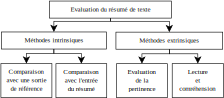
\includegraphics{evalRAT/classif-eval.pdf} % % %[width=140mm]
 \caption{Les approches d'évaluation des systèmes de résumé automatique.}
 \label{fig:classif-eval}
\end{center}
\end{figure}

\subsection{Évaluation intrinsèque}

\subsubsection{Critères utilisés}

Dans le but d'évaluer le résumé produit d'une manière intrinsèque, on compare le résumé produit par rapport au résumé de référence ou carrément avec le document source selon différents critère.
Le premier est la cohérence, qui consiste à la vérification de la lisibilité du résumé. 
Pour les résumés par extraction, les problèmes sont dus à la présence des anaphores et des brèches dans leurs structures rhétoriques. 
Pour les résumés par abstraction, les vérifications qu'on peut faire, d'après \cite{00-saggion-lapalme}, sont: la bonne orthographe et grammaire, l'indication claire sur le document source, style non personnel, la brièveté, la lisibilité et la compréhension, etc. 
Mais jusque-là, il est pratiquement impossible de procéder à une telle évaluation de manière automatique. 

L'autre critère est le contenu informatif du résumé, qui vise à estimer les informations que le résumé contient. 
Comme le résumé est plus court que le texte original, il y a moins d'informations préservées. 
Ainsi, la mesure du contenu informatif d'un résumé consiste à estimer la quantité d'information préservée par rapport au texte source. 

\subsubsection{Comparaison avec une sortie de référence}

L'idée est de comparer le résumé automatique avec celui fait par un humain d'un même texte source. 
L'évaluation classique de \cite{69-edmundson} a été réalisée par humain en comparant le résumé par machine avec celui crée par un humain. 
Le problème pour l'évaluation humain est que, même si on peut trouver plusieurs résumés de référence pour un même document, le système peut générer un résumé qui est différent de tous ces résumés de référence, mais qui est informatif et cohérent \cite{01-mani}. 
Dans une expérience conduite par \cite{61-rath-al}, où on a demandé aux humains d'extraire 20 phrases à partir de 10 articles scientifiques, on a trouvé que les juges ont produit des résumés différents pour la même source. 
En plus, on a trouvé que pour un même juge, celui-ci peut produire deux résumés totalement différents en un intervalle de huit semaines.
On peut aussi évaluer un résumé de manière automatique, en utilisant des différentes mesures, parmi elle ROUGE (va être détaillée ultérieurement).

\subsubsection{Comparaison avec l'entrée de résumé}

Dans ce type d'évaluation, le résumé et la source sont donnés à des personnes, en leurs demandant d'évaluer le contenu informatif du résumé dans le contexte de la source.
Selon \cite{01-mani} il existe deux types de méthodes pour la comparaison entre le résumé et la source: les méthodes sémantiques et les méthodes de surface.
Les méthodes sémantiques consistent à comparer le sens dans le texte source par rapport à celui du résumé. 
Une méthode est de marquer le sens de chaque phrase dans le résumé, ensuite voir combien de propositions existantes dans la source ce résumé couvre. 

Une méthode sémantique plus pratique se trouve dans l'approche de l'extraction d'information de \cite{93-paice-jones}. 
Pour évaluer leur outil de résumé, chaque texte est caractérisé par ses concepts focaux et non focaux. 
Les auteurs ont mesuré la couverture de ces concepts dans un résumé en termes de satisfaisant, non satisfaisant, insuffisant.
Dans les méthodes de surface, on ne cherche pas à représenter les concepts dans un niveau très profond, et donc il suffit de juger si les idées principales dans la source sont couvertes par le résumé. 
Une variante de ce type de méthode a été portée dans TIPSTER SUMMAC \cite{99-mani-al}; une tâche Q\&A (Question and Answer) pour l'évaluation des résumés automatiques. 
Dans cette tâche les passages dans le texte source ont été marqués en se basant sur le critère de pertinence à un sujet. 
Considérant un document et un sujet, un résumé concentré sur un sujet pour ce document est juste lorsqu'il contient des réponses pour les questions qui couvent l'information indispensable dans n'importe quel document jugé pertinent au sujet.

\subsection{Évaluation extrinsèque}

L'idée d'une évaluation extrinsèque d'un résumé est de déterminer l'effet de résumé sur d'autres tâches. 
Il existe plusieurs tâches sur lesquels un résumé peut être appliqué, parmi ces tâches on peut citer celles mentionnées dans \cite{01-mani}:
\begin{itemize}
\item Si le résumé affecte le comportement d'autres tâches, il est possible de mesurer l'efficacité en exécutant ces tâches. 
Par exemple, si on a un système de décision qui se base sur notre système de résumé automatique, on peut mesurer l'efficacité de notre système de résumé en examinant son effet sur le système de décision.
\item On peut examiner l'utilité de résumé avec respect des informations de besoin ou d'objectif, comme trouver des documents pertinentes au besoin d'une personne issus d'une large collection.
\item On peut évaluer l'impact d'un résumé sur le système qu'il le contient, par exemple, comment un outil de résumé peut aider dans un système de question-réponse?
\end{itemize}

\subsubsection{Évaluation de la pertinence}

Dans l'évaluation de la pertinence, on présente à une personne un document et un thème, et on lui demande de déterminer le rapport entre le document et le thème. 
L'influence de résumé sur la justesse et le temps dans la tâche est donc étudiée. 
Malgré que l'évaluation SUMMAC inclue une évaluation Q\&A intrinsèque, son principal attention est sur une évaluation extrinsèque. 
En utilisant un document (qui peut être un résumé ou un texte normal, l'évaluateur ne sais pas apriori sa nature), et une description d'un thème, l'évaluateur humain est amené à juger de la pertinence du document par rapport au thème. 
Il doit, donc, choisir une seule catégorie depuis cinq catégories (chacune a une description avec) qui exprime le thème de document, ou non en choisissant "\textit{aucune catégorie}". 

\subsubsection{Lecture et compréhension}

Dans la tâche de lecture et compréhension, l'évaluateur humain lit d'abord les sources et/ou les résumés assemblés d'un ou plusieurs documents. Il répond sur un test de choix multiples sur le contenu des documents. 
Ensuite, le système calcule le pourcentage des réponses correctes. 
De ce fait, une compréhension humaine basée sur un résumé peut être objectivement comparée avec celle basée sur la source. 
Le raisonnement est donc: si la lecture d'un résumé permet à une personne de répondre à des questions comme s'il a lu la source, le résumé est très informatif.

\section{Mesures intrinsèques populaires}

Les mesures varient selon le type de méthode utilisée: intrinsèque ou extrinsèque. 
La figure \ref{fig:intrin-mesures}, représente les mesures intrinsèques les plus utilisés dans le résumé automatique de texte. 
%
\begin{figure}[ht]
\begin{center}
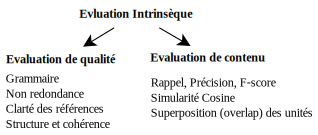
\includegraphics{evalRAT/intrin-mesures.pdf} % % %[width=140mm]
 \caption{Les mesures populaires dans l'évaluation intrinsèque.}
 \label{fig:intrin-mesures}
\end{center}
\end{figure}

\subsection{Évaluation de qualité}

Pour vérifier la qualité (linguistique) d'un texte, il existe des divers aspects:
\begin{itemize}
\item Grammaire: Il faut que le texte soit correct grammaticalement.
\item Non redondance: pas d'information redondante.
\item Clarté des références: Il faut que les liens anaphoriques (relation entre les noms et les pronoms) soient corrects.
\item Structure et cohérence: Le résumé doit avoir une bonne structure avec des phrases cohérentes.
\end{itemize}
Pour attribuer un score à chacun de ces scores, on utilise des évaluateurs humains.
La note peut être, par exemple, un caractère entre A (très bien) et E (très mauvais).

\subsection{Évaluation du contenu}

\subsubsection{Rappel, précision, et F-score}

C'est les mesures les plus utilisées pour juger la performance d'un système de la recherche d'information \cite{08-manning-al} et résumé automatique en particulier. 
Si nous avons un système du résumé automatique qui prend texte d'entrée ($E$), et produit un résumé comme sortie ($S$), et si nous avons un résumé de référence comme modèle ($M$), les relations entre ces documents sont comme suite:
\begin{itemize}
\item TP (true positive): qui est l'information jugée pertinente par $M$ et $S$, donc $M \cap S$.
\item TN (true negative): qui est l'information jugée non pertinente par $M$ et $S$, donc $E - (M \cup S)$.
\item FP (false positive): qui est l'information jugée pertinente par $M$ et non pertinente par $S$, donc $M - S$.
\item FN (false negative): qui est l'information jugée non pertinente par $M$ et pertinente par $S$, donc $S - M$.
\end{itemize}
La figure \ref{fig:mesures} représente ces différentes relations.
%
\begin{figure}[ht]
\begin{center}

\includegraphics{evalRAT/mesures.pdf} % % %[width=140mm]
 \caption{La relation entre les documents d'entrée, de sortie, et modèle.}
 \label{fig:mesures}
\end{center}
\end{figure}

Le rappel ($R$) représente le pourcentage des éléments pertinents sélectionnés par le système. 
Il est calculé en divisant le nombre des unités communes entre le résultat du système et le résultat attendu, par le nombre des unités composant le résultat attendu. 
Les unités peuvent être des phrases, des mots, etc. 
En utilisant les deux concepts $TP$ et $FN$, on peut exprimer le rappel comme dans l'équation \ref{eq:recall}.
\begin{equation}
\label{eq:recall}
R = \frac {TP} {TP + FN}
\end{equation}

La précision ($P$) représente le pourcentage des éléments sélectionnés qui sont corrects. 
Il est calculé en divisant le nombre des unités communes entre le résultat du système et le résultat attendu, par le nombre des unités composant le résultat du système. 
Les unités peuvent être des phrases, des mots, etc. 
En utilisant les deux concepts $TP$ et $FP$, on peut exprimer le rappel comme dans l'équation \ref{eq:precision}.
\begin{equation}
\label{eq:precision}
P = \frac {TP} {TP + FP}
\end{equation}

Le F-score est un mesure qui combine la précision et le rappel. 
Il est calculé en utilisant une moyenne harmonique entre la précision et le rappel, il est représenté par l'équation \ref{eq:f-score}.
\begin{equation}
\label{eq:f-score}
F_{\beta} = \frac
{(1+\beta^2) P \times R}
{ \beta^2 P + R}
\end{equation}
Le F-score le plus utilisé est le $F_1-score$ en remplaçant $\beta$ par $1$ ce qui nous donne une moyenne harmonique équilibre entre la précision et le rappel.
Lorsque $\beta > 1$, on va favoriser la précision, et lorsque $\beta < 1$ on va favoriser le rappel.

\subsubsection{Similarité de Cosinus}

La similarité cosinus permet de calculer la similarité entre deux vecteurs en déterminant l'angle entre eux. 
L'équation \ref{eq:cosine3} donne la méthode de calcul de similarité Cosinus.
\begin{equation}
\label{eq:cosine3}
cos(X,Y) = 
\frac {X . Y}{||X|| . ||Y||} = 
\frac {\sum_i {x_i.y_i} }{\sqrt{\sum_i(x_i)^2} . \sqrt{\sum_i(y_i)^2}}
\end{equation}
Où: 
X et Y sont deux vecteurs représentant une unité (texte, paragraphe, phrase, mot) du résumé de système et une unité du résumé de référence.

Dans le cas de recherche d'information, la similarité Cosinus de deux documents va être entre 0 et 1, puisqu'on utilise les fréquences des termes qui ne peuvent pas être négatives. 
Donc, l'angle entre deux vecteurs des fréquences des termes va être entre 0\textdegree et 90\textdegree. 
Plus l'angle entre deux vecteurs est petit, plus ils sont similaires. 

%\subsubsection{Superposition (overlap) des unités}
%
%\begin{equation}
%\label{eq:overlap}
%overlap(X,Y) = \frac {||X \cap Y||}
%{||X|| + ||Y|| - ||X \cap Y||}
%\end{equation}

\section{Méthodes d'évaluation}

\subsection{ROUGE}

ROUGE\footnote{ROUGE: Recall-Oriented Understudy for Gisting Evaluation} développé par \cite{03-Lin-hovy} est une méthode inspirée d'une autre méthode d'évaluation des systèmes de traduction automatique, appelée BLEU\footnote{BLEU: BiLingual Evaluation Understudy} \cite{02-papineni-al}. 
L'objectif est de déterminer automatiquement la qualité d'un résumé en le comparant par un autre résumé de référence créé par un humain. 
Le principe est de compter le nombre des unités de recouvrement comme les n-grammes, les séquences de mots, et les mots assemblés entre un résumé généré par ordinateur et le résumé de référence. 
La méthode ROUGE est une méthode basée sur le mesure de rappel puisque le dénominateur est le nombre des n-grammes contenant dans le résumé de référence, par contre la méthode BLEU utilise la mesure de la précision.
La méthode ROUGE contient cinq variantes \cite{04-lin}: ROUGE-N, ROUGE-L, ROUGE-W, ROUGE-S, et ROUGE-SU. 

\subsubsection{ROUGE-N}

ROUGE-N, formellement, est un rappel de n-grammes entre le résumé candidat et un ensemble de résumés de référence. 
La valeur de ROUGE-N peut être calculée par l'équation \ref{eq:rouge-n}. 
\begin{equation}
\label{eq:rouge-n}
ROUGE-(N) = \frac{\sum_{S \in Summ_{ref}}{\sum_{N-gram \in S}{Count_{match} (N-gram)}}}
{\sum_{S \in Summ_{ref}}{\sum_{N-gram \in S}{Count (N-gram)}}}
\end{equation}
Où, \textit{N} est la longueur du N-gramme, $count_{match}(N-gram)$ est le nombre des N-grammes du résumé candidat retrouvées dans un des résumés de référence ($Summ_{ref}$).
$Count (N-gram)$ est le nombre des N-grammes dans le résumé de référence. 

\subsubsection{ROUGE-L}

ROUGE-L utilise la sous-séquence commune la plus longue (LCS\footnote{LCS: Longest Common Subsequence}) entre deux phrases $ X $ avec $m_x$ mots et $ Y $ avec $n_y$ mots, pour estimer la similarité entre ces deux phrases (voir l'équation \ref{eq:lcs}). 
Pour appliquer LCS dans l'évaluation du résumé, il faut voir les phrases de ce résumé comme une séquence de mots. 
Sachant que la séquence commune la plus longue (LCS) ne suppose pas l'appariement consécutif entre les deux séquences. 
\begin{equation}
\label{eq:lcs}
R_{lcs}= \frac {\sum_{i=1}^u {LCS(X, Y)}}{m_x}, 
P_{lcs}= \frac {\sum_{i=1}^u {LCS(X, Y)}}{n_y}
\end{equation}
Pour comprendre mieux comment calculer ROUGE-L, voici un exemple d'une phrase de référence (r1) et deux phrases candidates (c1, c2):
\begin{description}
\item[r1] [\textit{A B C D}].
\item[c1] [\underline{A} E \underline{C D}].
\item[c2] [\underline{C D} E A].
\item[c3] [\underline{C D} \underline{\textit{A B}}].
\end{description}
ROUGE-L de c1 va être 3/4, et de c2 va être 2/4. 
Donc c1 est mieux que c2 selon ROUGE-L. 
Le problème de ROUGE-L est qu'elle calcule seulement la séquence principale, et donc autres LCS alternatifs ou moins longs ne vont pas être considérés dans le calcul du score. 
Dans la phrase c3, LCS compte seulement une séquence et pas les deux, et donc la valeur de ROUGE-L de c3 va être égale à celui de c2.

L'équation \ref{eq:rouge-l} représente la méthode de calcul de ROUGE-L (rappel et précision) entre un résumé de référence $r_i \in R$ et un résumé candidat $C$. 
\begin{equation}
\label{eq:rouge-l}
R_{lcs}= \frac {\sum_{i=1}^u {LCS_{\cup}(r_i, C)}}{m}, 
P_{lcs}= \frac {\sum_{i=1}^u {LCS_{\cup}(r_i, C)}}{n}
\end{equation}
Où:
\begin{itemize}
\item $u$ est le nombre des phrases dans le résumé de référence $R$. 
\item $LCS_{\cup}(r_i, C)$ est le score LCS de l'union des plus longues séquences entre la phrase de référence $r_i$ et les phrases du résumé candidat $C$. Par exemple:
\begin{quote}
Supposant une phrase de référence $r_i = w_1 w_2 w_3 w_4 w_5$, et $C$ contient deux phrases: $c_1 = w_1 w_2 w_6 w_7 w_8$ et $c2 = w_1 w_3 w_8 w_9 w_5$. 
Donc, le LCS entre $r_i$ et $c_1$ est "$w_1 w_2$", et le LCS entre $r_i$ et $c_2$ est "$w_1 w_3 w_5$";
L'union de ces deux LCS nous donne "$w_1 w_2 w_3 w_5$" et $LCS_{\cup}(r_i, C)= 4/5$.
\end{quote}
\item $m$ est le nombre des mots dans $R$, et $n$ est le nombre des mots dans $C$. 
\end{itemize}

\subsubsection{ROUGE-W}

Malgré les bonnes propriétés du LCS notées auparavant, il souffre du problème de différenciation entre les sous-séquences communes ayant des différentes relations spatiales dans leurs séquences originales.
Par exemple, si on a une séquence de référence r1 et deux séquences candidates c1 et c2 comme suit:
\begin{description}
\item[r1] [\underline{A} \underline{B} \underline{C} \underline{D} E F G]
\item[c1] [\underline{A} \underline{B} \underline{C} \underline{D} H I K]
\item[c2] [\underline{A} H \underline{B} K \underline{C} I \underline{D}]
\end{description}
c1 et c2 ont le même score ROUGE-L, mais dans ce cas c1 devrait avoir un score supérieure à celui de c2, puisqu'elle contient des appariements consécutifs. 
Pour améliorer la méthode de LCS, les appariements consécutifs sont accordés plus de score que les appariements non consécutifs. 
Ceci est accompli en pénalisant toute séquence non consécutive. 

L'équation \ref{eq:rouge-w} représente la méthode de calcul de ROUGE-W (rappel et précision) entre un résumé de référence $r_i \in R$ et un résumé candidat $C$. 
\begin{equation}
\label{eq:rouge-w}
R_{wlcs}= f^{-1}(\frac {WLCS(r_i,C)}{f(m)}), 
P_{wlcs}= f^{-1}(\frac {WLCS(r_i,C)}{f(n)})
\end{equation}
Où:
\begin{itemize}
\item $ f $ est une fonction satisfaisant la relation $ f(x,y)>f(x)+f(y) $. Prenant $ f(k) = k^2 $ où $ k $ est la taille d'une LCS.
\item $WLCS(r_i,C) = \sum_j f(LCS_j(r_i,C))$, $LCS_j(r_i,C)$ est la taille de LCS numéro $ j $ entre la phrase de référence $r_i$ et les phrases du résumé candidat $C$. Par exemple:
\begin{quote}
Dans l'exemple précédent, c1 donne une seule LCS: "A B C D". 
Donc, $ ROUGE-W(c1) = \sqrt{(4^2)}/7 = 0.57143 $. 

Pour la deuxième séquence c2, on a quatre LCS: "A", "B", "C", et "D". 
Donc, $ ROUGE-W(c2) = \sqrt{(1^2 + 1^2 + 1^2 + 1^2)}/7 = 0.28571 $. 
\end{quote}
\item $m$ est le nombre des mots dans $R$, et $n$ est le nombre des mots dans $C$. 
\end{itemize}

\subsubsection{ROUGE-S}

ROUGE-S\footnote{ROUGE-S: skip-bigram co-occurrence} est une extension de ROUGE-N; elle est calculée de la même manière que ROUGE-2, sauf qu'elle utilise les bi-grammes à trous au lieu des bi-grammes consécutives. 
Le bi-gramme à trous (skip bigram), comme défini dans \cite{04-lin}, est n'importe quelle paire de mots dans leurs ordre dans la phrase, qui permettent des trous arbitraires. 
Si on a $X$ un texte de référence avec $m$ mots et $Y$ un texte candidat avec $n$ mots, on peut calculer ROUGE-S comme suit.
\begin{equation}
\label{eq:rouge-s}
R_{SKIP2}(X, Y) = \frac {SKIP2(X, Y)}{C(m, 2)}, 
P_{SKIP2}(X, Y) = \frac {SKIP2(X, Y)}{C(n, 2)}
\end{equation}
Où $SKIP2(X,Y)$ est le nombre des bi-grammes à trous semblables entre $X$ et $Y$.
$C$ est la fonction de combinaison.

Prenant l'exemple utilisé dans ROUGE-L, où r1 est la phrase de référence et les trois phrases c1, c2, et c3 sont les phrases candidates: 
\begin{description}
\item[r1] [\textit{A B C D}].
\item[c1] [A E C D].
\item[c2] [C D E A].
\item[c3] [C D A B].
\end{description}
Chaque phrase contient $C(4,2)=6$ bi-grammes à trous. 
Par exemple la phrase c1 a les bi-grammes suivants: ("A E", "A C", "A D", "E C", "E D", "C D"). 
Le score ROUGE-S pour c1, c2, et c3 sont: 3/6, 1/6, et 2/6 respectivement.

\subsubsection{ROUGE-SU}

Un problème de ROUGE-S est qu'elle ne donne aucun crédit pour une phrase candidate si cette phrase ne contient aucune paire de mots semblables à ceux de la phrase de référence.
Par exemple, la phrase suivante donne un score ROUGE-S à zéro:
\begin{description}
\item[c4] [D C B A].
\end{description}
Cette phrase est l'inverse de la phrase r1 et il n'existe aucun bi-gramme à trous similaire à ceux de r1. 
Pourtant, on veut faire la différence entre les phrases comme c4 et les phrases qui ne contiennent aucun mot en commun avec r1. 
Pour le faire, on peut étendre ROUGE-S avec l'addition des uni-grammes comme unités de calcule, ce qui nous donne ROUGE-SU.

Chaque phrase contient $C(4,2) + 4 = 10$ grammes. 
Par exemple la phrase c1 a les grammes suivants: ("A E", "A C", "A D", "E C", "E D", "C D", "A", "B", "C", "D"). 
Le score ROUGE-SU pour c1, c2, c3, et c4 sont: 7/10, 5/10, 6/10, et 4/10 respectivement.

\subsection{BE}

%Définir les BEs
Les éléments basiques (\textit{Basic Elements: BEs}) sont des unités sémantiques minimales qu'on peut obtenir d'une phrase. 
D'après \cite{06-hovy-al}, le problème d'évaluation du contenu d'un résumé peut être résolu en utilisant trois différents modules: découpeur de BE, comparateur de BE , et évaluateur de BE. 
Le premier sert à créer les unités BE d'un texte d'entrée, le deuxième sert à évaluer la similarité entre deux BE, et le troisième sert à donner un score pour chaque BE.

Le système d'évaluation utilisant les BEs prend le résumé et un ensemble des résumés de référence pour avoir un score. 
Il applique les trois modules précédents deux fois, en deux étapes: la préparation et la notation. 
Dans la phase de préparation, le premier module décompose les résumés de référence en une liste de BEs de référence; le second module prend en compte tous BEs de référence et fusionne ceux sémantiquement identiques et le troisième module attribue un score à chacun des BEs de référence.
Dans la deuxième étape (notation), le premier module décompose le résumé en une liste séparée de BEs, le second compare chaque BE à la liste des BEs de référence, le troisième attribue un score à chaque BE et calcule le score global de tous les BEs contenus dans le résumé candidat.

Le découpeur de BE est consacré pour décomposer un texte sur des BEs, en utilisant une des règles de découpage construites manuellement exécutées sur l'arbre syntaxique du texte d'entrée. 
Des expérimentations sont conduites par \cite{06-hovy-al} pour définir les BEs comme suit:
\begin{itemize}
\item l'entête d'un constituant syntaxique majeur (nom, verbe, adjectif, ou phrase adverbiale) exprimé comme un élément seul, ou
\item une relation entre un BE d'entête et un dépendant simple, exprimé comme un triple (entête, modificateur, relation).
\end{itemize}

%comparaison des BEs
Le comparateur sert à comparer deux BEs en utilisant des stratégies de comparaison. 
Les stratégies de comparaison sont catégorisées sur plusieurs classes (de la plus simple à la plus complexe):
\begin{itemize}
\item Similitude lexicale: les mots doivent être comparables exactement.
\item Similitude de lemmes: les formes racines des mots doivent être comparables.
\item Similitude de synonyme: les mots ou leurs synonymes identifiés par WordNet, doivent être comparables exactement.
\item Les paraphrases doivent être comparables (une approximation).
\item La généralisation sémantique: les mots construisant les BEs sont remplacés par leurs généralisations sémantiques ("Peugeot" sera remplacé par "voiture") puis comparés dans une diversité des niveaux d'abstraction.
\end{itemize}

%Donner un score pour les BEs
L'évaluateur sert à donner un score à chaque BE. 
Dans \cite{06-hovy-al}, les auteurs ont attribué à chaque BE un (1) point à chaque fois qu'il participe à un résumé de référence. 
Ce score est attribué en se basant sur la similarité entre le BE et les BEs de référence.
Le score global est la somme des poids des BEs qui figurent dans le résumé candidat.

\subsection{Pyramides}

L'évaluation de similarité entre le résumé automatique et le résumé humain, se fait en utilisant des métriques comme la précision et le rappel. 
Mais, selon \cite{07-nenkova-al}, cette méthode présente quelques inconvénients: 
\begin{itemize}
\item La variation humaine: différentes personnes peuvent sélectionner des phrases différentes à intégrer dans le résumé. 
Même pour une personne, elle peut produire deux résumés différents. 

\item Granularité de l'analyse: Même si le système ne choisit pas exactement la même phrase que le résumé modèle, cette phrase peut être pertinente avec une ou plus de phrases du modèle. 
L'appariement partiel doit être pris en compte, mais il exige une analyse au-dessous du niveau phrase. 

\item L'équivalence sémantique: différentes phrases peuvent exprimer la même signification, même si elles n'utilisent pas les mêmes mots. 
Naturellement, les annotateurs doivent choisir seulement une phrase parmi les phrases équivalentes, et le système qui choisit une autre phrase équivalente doit être pénalisé. 

\item Extrait ou abstrait? Le résumé humain est un résumé par abstraction; une personne utilise ses propres mots pour rédiger un résumé. 
Ainsi, l'appariement exact entre les phrases de système et celle du modèle (fait par l'humain) n'est pas possible. 
\end{itemize}

La méthode Pyramides \cite{07-nenkova-al}, a été développée dont l'objectif est de remédier à ces problèmes.
Elle est une évaluation quantitative du contenu sélectionné par un système de résumé, qui nécessite un résumé de référence qu'on puisse utiliser pour évaluer le résumé généré automatiquement.
La pyramide est une représentation du résumé de référence attribué à chaque ensemble de documents d'entrée. 
Puisque le pyramide est utilisé pour évaluer le contenu du résumé, les unités de comparaison dans un pyramide correspondent aux unités de signification (sens), il sont appelées "\textit{summary content units (SCUs)}". 

Contrairement aux méthodes utilisant un résumé de référence, un pyramide représente les opinions de plusieurs résumeurs humains, qui ont écrit chacun un résumé modèle pour l'ensemble de documents d'entrée. 
La caractéristique clé d'un pyramide est qu'il quantifie l'accord entre les résumés humains. 
Les SCUs qui apparaissent dans plus de résumés humains vont avoir plus de score, ce qui nous permet de faire la différence entre le contenu plus important que celui moins important. 

Une fois l'annotation faite, les SCUs finaux sont partitionnés sur un pyramide en se basant sur les poids de ces SCUs. 
Chaque étage contient seulement les SCUs ayant le même poids. 
Le nombre \textit{n} des résumés modèles annotés, représente le nombre maximal d'étages dans un pyramide. 
La taille d'un pyramide (nombre d'étages) peut être différent de sa taille dans le cas où il n'y a pas une superposition entre tous les modèles utilisés dans la création de pyramide. 
Il y a un petit nombre de SCUs (dans la sommet de pyramide), que tout le monde ont exprimé dans leurs résumés, et un trop large nombre de SCUs exprimés par un seul résumé modèle (dans la base de pyramide). 
Donc, en descendant dans le pyramide, les SCUs deviennent moins importants dans leurs informations, vu qu'ils apparaissent dans moins de résumés. 
La figure \ref{fig:meth-pyramids} représente un pyramide avec deux SCUs dans le sommet et quatre dans l'étage suivant, elle illustre deux  parmi six résumés optimaux de taille 4 SCUs que ce pyramide prévoit. 
\begin{figure}[ht]
\begin{center}
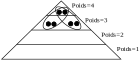
\includegraphics{evalRAT/meth-pyramids.pdf} % % %[width=140mm]
 \caption[Deux parmi six résumés optimaux avec 4SCU]{Deux parmi six résumés optimaux avec 4SCU \cite{07-nenkova-al}.}
 \label{fig:meth-pyramids}
\end{center}
\end{figure}

En se basant sur une pyramide, le contenu informatif du nouveau résumé peut être calculé comme le rapport entre la somme des poids de ses SCUs et le poids d'un résumé optimal avec le même nombre de SCUs. 
%\cite{07-nenkova-al} ont présenté une formule pour calculer le poids de résumé optimal (voir la formule \ref{eq:max-pyramids}). 
%\begin{equation}
%\label{eq:max-pyramids}
%Max = \sum_{i=j+1}^{n}{i\times |T_i|+j \times (X - \sum_{i=j+1}^{n}{|T_i|})} ; 
%j= \max_i{(\sum_{t=i}^{n}{|T_t|\geq X})}
%\end{equation}
%Où $n$ est le nombre des étage dans le pyramide, 
%$T_i$ est l'étage numéro $i$ (Le poids des SCUs dans l'étage $T_i$ égale à $i$), 
%$|T_i|$ est le nombre des SCUs dans l'étage $i$, 
%et $X$ est la taille du résumé en SCUs. 

\section{Campagnes d'évaluation}

\subsection{SUMMAC}

SUMMAC est la première conférence d'évaluation de résumé automatique\cite{99-mani-al}, elle est lancée par le gouvernement Américain en mai 1998. 
Trois tâches principales d'évaluation ont été définies: la tâche ad-hoc, la tâche de catégorisation, et la tâche question-réponse. 

Dans la tâche ad-hoc, le centre d'intérêt est les résumés indicatifs adaptés à un thème particulier. 
Pour un document (qui peut être un résumé ou un texte source, l'évaluateur ne sait pas), et une description d'un thème, on demande à l'évaluateur de déterminer si le document est pertinent pour le thème. 

Dans la tâche de catégorisation, l'évaluation cherche à trouver si un résumé générique peut aider un analyste de catégoriser un document rapidement et correctement. 
Ici, le thème n'est pas connu pour le système de résumé. 
Pour un document, qui peut être un résumé générique ou un texte source (l'évaluateur ne sait pas), le testeur doit choisir parmi cinq catégories données, celle pour laquelle le document est pertinent, sinon il choisit "\textit{aucune catégorie}". 

La tâche question-réponse implique l'évaluation du contenu informatif du résumé par rapport à un thème donné; c'est-à-dire le nombre de réponses qu'on peut trouver, en lisant le résumé, pour des questions reliées à ce thème et générées du document source. 
Chaque résumé est comparé manuellement à la réponse de référence pour un document donné, pour juger si la réponse de résumé est correcte, partiellement correcte, ou incorrecte.
Deux métriques d'exactitude sont utilisés: ARS (\textit{Answer Recall Strict}) et ARL (\textit{Answer Recall Lenient}), représentés par l'équation \ref{eq:answer-recall}.
\begin{equation}
\label{eq:answer-recall}
ARS = \frac{n1}{n3}, 
ARL = \frac{n1 + (.5 * n2)}{n3}
\end{equation}
Où $ n1 $ est le nombre des réponses correctes dans le résumé, $ n2 $ est le nombre des réponses partiellement correctes, et $ n3 $ est le nombre des questions répondues dans la réponse de référence.

\subsection{DUC/TAC}

DUC\footnote{DUC site web: \url{http://duc.nist.gov/}} (Document Understanding Conference) est une série d'évaluations organisée par NIST\footnote{NIST: National Institute of Standards and Technology} dans le cadre du projet TIDES\footnote{TIDES: DARPA's Translingual Information Detection, Extraction, and Summarization.}. 
Il a comme but de faire évaluer la technologie des résumés automatique en permettant aux chercheurs de participer à des expériences à grande échelle. 
Dans DUC 2004, il y avait 5 tâches d'évaluation:
\begin{itemize}

\item \textbf{La tâche 1 - résumés très courts mono-document:} Pour chaque document des 50 documents en Anglais, il faut créer un résumé très court (<=75 octets).

\item \textbf{La tâche 2 - résumés courts multi-document:} Pour chaque groupe des 50 groupes de documents en Anglais, il faut créer un résumé court (<=665 octets).

\item \textbf{La tâche 3 - résumés très courts mono-document trans-linguistique:} Pour chaque translation en Anglais (automatique et manuelle) des 25 documents en Arabe, il faut créer un résumé très court (<=75 octets).

\item \textbf{La tâche 4 - résumés courts multi-document trans-linguistique:} Pour chaque groupe de translations en Anglais (automatique et manuelle) des 25 groupes de documents en Arabe, il faut créer un résumé court (<=665 octets).

\item \textbf{La tâche 5 - résumés courts guidés par une requête:} Pour chaque groupe des 50 groupes de documents en Anglais, il faut créer un résumé court (<=665 octets) pour répondre à une question au forme "\textit{Who is X?}", où X est le nom d'une personne ou groupe de personnes.

\end{itemize}
Les résumés qui dépassent la taille limite vont être tronqués, et aucun bonus ne va être attribué aux résumés plus courts. 
L'évaluation des tâches 1-4 est faite en utilisant ROUGE (ROUGE-1, ROUGE-2, ROUGE-3, ROUGE-4, et ROUGE-L). 
Pour la tâche 5, les résumés sont évalués, d'une façon intrinsèque, en terme de qualité et de couverture en utilisant le système SEE\footnote{SEE: Summary Evaluation Environment (\url{http://www.isi.edu/licensed-sw/see/})}. 
En terme de pertinence vis-à-vis la question "\textit{Who is X?}", ils sont évalués par des évaluateurs humains.

Dans DUC 2007, les documents utilisés pour le résumé sont ceux du corpus AQUAINT, contenant des articles hebdomadaire diversifiés de \textit{Associated Press} et \textit{New York Times} (1998-2000) et \textit{Xinhua News Agency} (1996-2000).
Il y avait 2 tâches: tâche principale et tâche de mise-à-jour.
\begin{itemize}
\item \textbf{Tâche principale:} En fournissant 25 documents et un thème, la tâche est de synthétiser un résumé courant et bien organisé de 200 mots afin de répondre à une ou plusieurs questions. 

\item \textbf{Tâche de mise-à-jour:} le but est de produire des résumés courts multi-documents (environ 100 mots) de mise-à-jour en supposant que l'utilisateur a déjà lu l'ensemble des articles précédents.
\end{itemize}
Pour la première tâche, l'évaluation est conduite comme suit:
\begin{itemize}
\item la forme linguistique est évaluée manuellement pour chaque résumé, en utilisant des critères de qualité: la grammaire, la non redondance, la clarté de références, la concentration, la structure et la cohérence. 
Pour chacun de ces critères, les évaluateurs donnent une note entre 1 (pas bon) et 5 (très bon). 

\item La pertinence vis-à-vis un thème donné, est évaluée manuellement pour chaque résumé en utilisant une note entre 1 (pas bon) et 5 (très bon).

\item Pour chaque résumé automatique, ROUGE-2 et ROUGE-SU4 sont calculés.

\item Pour chaque résumé automatique, BE est calculé.
\end{itemize}
Pour la deuxième tâche, chaque résumé va être évalué selon: ROUGE-2, ROUGE-SU4, BE, et Pyramides.

Depuis 2008, DUC a été inclus dans la conférence TAC comme une tâche nommée "le résumé guidé". 
La tâche de résumé guidé (\textit{guided summarization}) a comme but d'encourager les systèmes de résumé de faire une analyse linguistique (sémantique) plus profonde sur les documents sources que d'utiliser les fréquences de mots pour sélectionner les concepts. 
Dans TAC 2010, la tâche de résumé guidé est de générer un résumé de 100 mots pour un ensemble de 10 articles de presse pour un thème donné, où le thème appartient à une catégorie prédéfinie. 
Il y a cinq catégories des thèmes: les accidents et les catastrophes naturelles, les crises, la santé et de la sécurité, les ressources menacées, les enquêtes et les procès.
Pour un thème donné, la tâche est d'écrire 2 résumés (pour deux ensembles de documents A et B):
\begin{itemize}
\item Un résumé pour l'ensemble A est guidé par requête.
\item Un résumé guidé par requête pour l'ensemble B sachant que l'utilisateur du résumé a déjà lis les documents de l'ensemble A.
\end{itemize}
Chaque résumé doit couvrir des aspects définis pour son catégorie (par exemple, WHAT? WHY? WHEN? WHERE?). 
L'évaluation se fait sur le contenu, la lisibilité, et la sensibilité. 
Pour le contenu, le score est calculé par la méthode Pyramides. 
Pour la lisibilité et la sensibilité globale, des évaluateurs sont demandés de donner un score entre 1 (très mauvais) et 5 (très bon).

\subsection{NTCIR}

L'atelier NTCIR est une série d'évaluations désignée pour supporter la recherche dans les technologies d'accès à l'information, y compris la recherche d'information, les questions-réponses, le résumé de texte, l'extraction, etc. 
L'objectif de NTCIR est: 
\begin{enumerate}
\item D'encourager la recherche dans les technologies d'accès à l'information en fournissant des collections de test large-échelle utilisées pour les expériences et les évaluations. 
\item De fournir un forum pour les groupes de recherche qui s'intéressent à la comparaison entre systèmes et l'échange d'idées. 
\item D'examiner les méthodes d'évaluation des techniques d'accès d'information et les méthodes de construction de corpus de données large-échelle utilisées dans les expériences. 
\end{enumerate}

Dans le deuxième atelier de NTCIR (1999), le défi de résumé automatique de textes contient trois tâches. 
Les deux premières tâches sont pour l'évaluation intrinsèque (appelés tâche A) où les participants résument automatiquement des documents en spécifiant la longueur de résumé. 
La troisième tâche est pour l'évaluation extrinsèque (appelé tâche B) où les résumés sont évalués en conduisant une tâche de RI. 
Les processus de ces tâches sont comme suit \cite{01-fukusima-okumura}:
\begin{itemize}
\item \textbf{Tâche A-1:} dans cette tâche le but est d'extraire les phrases les plus importantes. 
Le taux de résumé est défini comme la proportion entre le nombre des phrases choisies et le nombre total des phrases dans l'article. 
Les taux utilisés dans cette tâche sont 10\%, 30\%, 50\%.

\item \textbf{Tâche A-2:} dans cette tâche le but est de produire des résumés (par abstraction) en simple texte pour être comparés avec les résumés préparés par les humains. 
Le taux de résumé est défini comme la proportion entre le nombre des caractères dans le résumé et le nombre total des caractères dans l'article. 
Les taux utilisés dans cette tâche sont environ 20\% et 40\%. 

\item \textbf{Tâche B:} dans cette tâche le but est de produire des résumés en se basant sur des requêtes et des documents trouvés selon ces requêtes. 
Pour chacun de ces documents, il faut produire un résumé (pas un résumé multi-documents). 
La longueur du résumé n'est pas limitée, mais les résumés doivent être en un texte simple (sans marquages HTML, XML, etc.). 
\end{itemize}

Pour les documents utilisés, des experts sont demandés de sélectionner les phrases les plus importantes dans chaque document source pour évaluer les résumés par extraction. 
Pour les résumés par abstraction, le résumé produit manuellement en utilisant deux manières; la première est de sélectionner les parties importantes dans les phrases extraites manuellement, la deuxième est de résumé le document librement. 
L'évaluation des tâche se fait comme suit \cite{01-fukusima-okumura}:
\begin{itemize}
\item \textbf{Tâche A-1:} On cherche les phrases correctes dans le résumé.
Ensuite, on calcule les métriques: rappel, précision, et f1-score pour chaque résumé en prenant le nombre des phrases comme unité de calcule pour ces métriques. 
Le score final est la moyenne des scores de tous les résumés. 

\item \textbf{Tâche A-2:} Dans cette tâche, l'évaluation se fait selon deux manières: l'évaluation basée sur le contenu et l'évaluation subjective. 
Dans la première évaluation, les résumés système ainsi que les deux types de résumé humains sont analysés morphologiquement pour extraire des vecteurs contenant les mots de contenu, ensuite la distance entre le vecteur des fréquences de mots de résumé humain et de système est calculée. 
Dans la deuxième évaluation, on demande des juges humains d'évaluer les résumés selon deux critères la couverture et la lisibilité, en donnant une note entre 1 (très bien) et 4 (très mauvais). 
Les juges disposent de 4 résumés: les deux résumés humains, le résumé système, et un résumé produit en se basant sur la méthode LEAD. 

\item \textbf{Tâche B:} Dans cette tâche, les évaluateurs disposent des requêtes et des résumés des documents trouvés selon ces requêtes. 
Ils lisent les résumés et jugent la pertinence de ces documents vis-à-vis la requête. 
La méthode d'évaluation est essentiellement la même que celle de SUMMAC. 
Les mesures rappel, précision, et f1-score sont utilisés en prenant le nombre des documents comme unité pour ces mesures, ainsi que le temps nécessaire pour cette tâche. 
\end{itemize}

\section{Défis de l'évaluation} 

Selon Mani \cite{01-mani}, il existe plusieurs défis quant à l'évaluation des résumés automatiques:
\begin{itemize}
\item Le résumé implique une sortie produite par machine qui résulte dans la communication par langage naturel. 
Dans le cas où la sortie est une réponse à une question, il existe peut-être une réponse correcte, mais dans d'autres cas il est difficile d'arriver à définir c'est quoi une sortie correcte.
Il y a toujours la possibilité qu'un système génère un bon résumé qui soit tout-à-fait différent des résumés humains utilisés pour l'évaluation. 

\item Étant donné que c'est à un humain de juger de la sortie du système, ceci peut diminuer considérablement les charges d'une évaluation. 
Une évaluation utilisant un programme de score au lieu de jugements humains est préférable, puisque on peut la répéter facilement. 

\item Le résumé entraîne la compression, donc il est important d'évaluer les résumés dans des différents taux de compression. 
Ceci augmente l'échelle et la complexité d'une évaluation. 
Puisque le résumé implique la présentation de l'information adapté aux besoins des utilisateurs, la prise en compte de ces facteurs complique d'avantage le processus d'évaluation. 
\end{itemize}

\section{Conclusion}

Dans ce chapitre, nous avons présenté un état de l'art sur l'évaluation de résumé automatique. 
L'évaluation de résumé automatique et plus généralement les systèmes RI est un domaine de recherche eu lui-même, qui ne peut être décrit dans un chapitre. 
Dans un premier temps, nous avons défini les deux approches d'évaluation de résumé automatique: l'évaluation intrinsèque et l'évaluation extrinsèque. 
Pour évaluer un résumé, des mesures sont utilisés, parmi ces mesures nous avons cité les plus utilisés dans l'évaluation intrinsèque. 
Ces mesures évaluent la qualité linguistique de résumé, ainsi que le contenu informatif du résumé. 
Parmi les méthodes utilisées pour l'évaluation intrinsèque, nous avons cité: ROUGE, BE, et Pyramides, utilisés dans différentes campagnes d'évaluation: DUC/TAC, SUMMAC, et NTCIR. 
Finalement, nous avons mis les points sur les défis qui rendent l'évaluation à une tâche difficile à faire. 

%Dans le chapitre suivant
Dans le chapitre suivant, nous allons présenter notre système de résumé automatique basé sur l'approche statistique. 
L'idée principale est d'améliorer cette approche en introduisant le regroupement pour trouver les différents thèmes présents dans le document source. 
Ensuite en utilisant un algorithme d'apprentissage, nous avons créé un modèle pour chaque thème. 
En utilisant ces modèles, on cherche à trouver les phrases qui peuvent représenter tous (ou la plupart) des thèmes. 

%========================Le pied de chapitre=======================================
%==================================================================================
\ifx\wholebook\relax\else
 \cleardoublepage
 \bibliographystyle{../use/ESIbib} %../includes/ThesisStyle
 \bibliography{../bib/evalRAT} %,../bib/yay
 \end{document}
\fi
%==================================================================================
